\problemname{Bonsai}

De fleste der dyrker bonsai, siger at de gør det, fordi det er »vanskeligt« eller »harmonisk«.
Det er nu ikke derfor, Tina gør det.
Hun vil bare score kassen på at sælge træerne, så hun får råd til at købe en masse jamaicaæbler.
Hun har lige sat en ny knold i jorden og er begyndt at drømme om det næste jamaicaæble.
Hvor mange år skal hun mon vente, til hun har fremavlet det bonsaitræ, hendes kunde ønsker sig?

Bonsaitræer består af $2\leq N \leq 10^5$ knolde og $N-1$ grene.
Knuderne er nummereret fra $0$ til $N-1$. 
Alle bonsaitræer begynder med en lille knold som man sætter ned i jorden.
Hvert år vokser der en ny gren ud fra hver knold, og i grenens ende dannes en ny knold.
Man kan klippe grene af træet når som helst. 
Tina minder dig om, at det ikke spiller nogen rolle, hvor i træet roden sidder.

Givet kundens beskrivelse af et træ hvor mange år skal Tina vente, inden hun har fremavlet sådan et træ?

\section*{Indlæsning}

Første linje indeholder et heltal $2\leq N\leq 10^5$, antallet af knolde i det ønskede bonsaitræ.
De næste $N$ linjer beskriver bonsaitræet på følgende måde:
På linje $i$ står først et heltal $0 < m_i < N$, antallet af grene udgående fra den $i$te knold. 
Derefter følger $m_i$ heltal, som angiver de knolde der sidder sammen med den $i$te knold.

\section*{Udskrift}

Et heltal $A$: antallet af år det tager Tina at fremavle det bonsaitræ, som kunden beskriver.

\section*{Pointgivning}

Din løsning bliver kørt på seks grupper af test.
For at få point for en gruppe, skal du klare alle test i gruppen. 

\medskip\noindent
\begin{tabular}{ l  l  l }
Gruppe & Point      & Begrænsninger \\ \hline
1      &  9         & $m_i\leq 2$ og det er bedst at lade træet gro fra knude~0.\\ 
2      & 11         & $m_i \leq 3$ og det er bedst at lade træet gro fra knude~0. \\ 
3      & 18         & $A \leq 15$ og det er bedst at lade træet gro fra knude~0. \\ 
4      & 22         & Det er bedst at lade træet gro fra knude~0. \\ 
5      & 12         & $N \leq 250$. \\
6      & 28         & Ingen yderligere begrænsninger. 
\end{tabular}

\section*{Forklaring af eksempel 1}
Tina kan fremavle træet på to år ved at lade det vokse som i nedenstående figur.

\[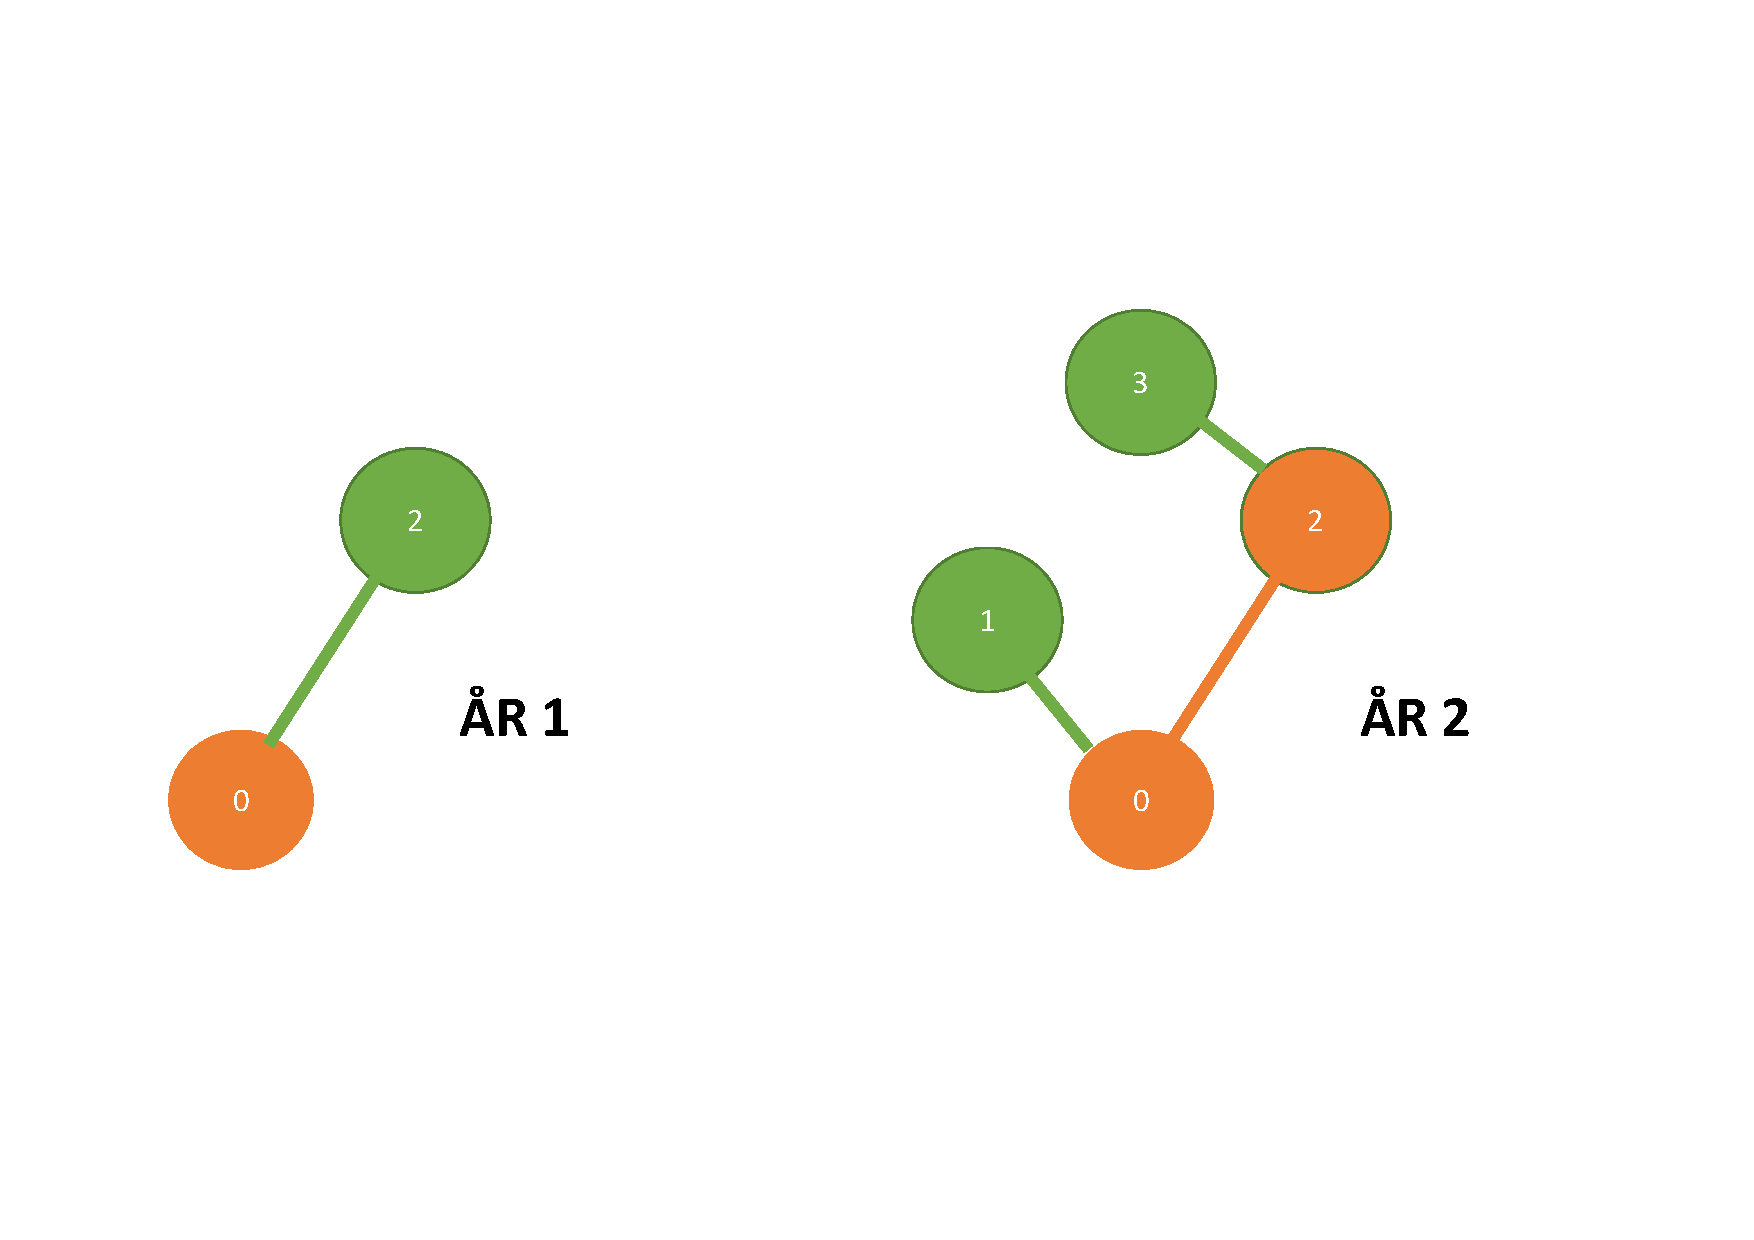
\includegraphics[width=0.5\textwidth]{Bonsaitree}\]
